\chapter{Инвариантные законы, четырёхвекторы и тензор поля}

Мы начнём с закона, которому природа могла бы подчиняться, но не подчиняется. Его несостоятельность подскажет нам, как следует записывать физический закон. Тот же критерий сначала ведёт от координатных компонент к обычным векторам, затем от обычных векторов к четырёхвекторам и, наконец, от четырёхвекторов к тензорам. К концу обсуждения электрическое и магнитное поля уже не будут отдельными объектами: вместе они займут шесть независимых компонент одного антисимметричного тензора.

Если не оговорено иное, мы используем единицы, в которых \(c=1\), упорядочиваем компоненты пространства-времени как \((1,2,3,0)=(x,y,z,t)\) и используем сигнатуру метрики \((-,-,-,+)\).

\section{Возможный закон с неправильной симметрией}

Жёстко закрепим в пространстве оси \(x\) и \(y\). Теперь постулируем, что две частицы взаимодействуют всякий раз, когда совпадают их \(x\)-координаты. Взаимодействие может обратить их движение или отбросить их в новых направлениях; его детальная динамика несущественна. Предлагаемое условие срабатывания просто таково:
\begin{equation}
  x_1-x_2=0,
\end{equation}
где нижние индексы обозначают частицы, а не компоненты координат. В этом правиле нет никакого математического противоречия. Вопрос в том, что делает его физически неправдоподобным.

\begin{classroomqa}
\audiencequestion{Нарушает ли это правило однородность пространства?}
\lecturerresponse{Нет. Перенос начала координат изменяет обе координаты на одну и ту же величину и оставляет \(x_1-x_2\) неизменным. Правило не задаёт никакого предпочтительного места. Его недостаток связан с изотропией: оно выделяет одно предпочтительное направление.}
\end{classroomqa}

Повернём оси на \(90^\circ\). Старое направление \(x\) теперь называется \(y\), так что те же физические события описывались бы равенством \(y\)-координат. При произвольном угле условие включало бы линейную комбинацию \(x\) и \(y\). Следовательно, форма закона зависит от того, как была ориентирована доска. Он инвариантен относительно переносов, но не инвариантен относительно вращений.

Обычно мы придаём физическим законам их наиболее простой вид в ортогональных координатах. Можно пользоваться и более общими координатами, но тогда метрика и формулы становятся менее простыми. В классе ортогональных декартовых систем отсчёта никакая ориентация не должна быть привилегированной.

Исправление напрашивается сразу. В двумерном случае нужно требовать совпадения обеих координат; в трёхмерном случае — всех трёх:
\begin{equation}
  x_1=x_2,
  \qquad y_1=y_2,
  \qquad z_1=z_2.
\end{equation}
Тогда частицы могут взаимодействовать только тогда, когда достигают одной и той же точки, даже если они подходят к ней по разным линиям.

\begin{classroomqa}
\audiencequestion{Должны ли также совпадать \(z\)-координаты и времена?}
\lecturerresponse{В трёхмерном пространстве должны совпадать и \(z\)-координаты. Время пока опускается; мы вернём его, как только пространственный аргумент будет завершён.}
\end{classroomqa}

Пусть \(\boldsymbol r_a\) — положение частицы \(a\). Три покомпонентных условия превращаются в одно векторное уравнение,
\begin{equation}
  \boldsymbol r_1-\boldsymbol r_2=\boldsymbol 0.
\end{equation}
Компонента может обращаться в нуль в одной повёрнутой системе координат и не обращаться в нуль в другой. С целым вектором дело обстоит иначе: если в одной системе координат каждая компонента равна нулю, то и в любой повёрнутой системе координат каждая компонента равна нулю. Точно так же, если два вектора равны в одной системе координат, они остаются равными после преобразования обоих.

\begin{figure}[H]
\centering
\includegraphics[width=0.78\textwidth]{lecture_06_figure_01.png}
\caption{Три равенства координат, благодаря которым столкновение означает пространственное совпадение, а не совпадение вдоль одной предпочтительной оси.}
\lectureframe{00:09:00}
\end{figure}

Вот почему векторные уравнения полезны. Их компоненты меняются, но сам объект преобразуется согласованно. Закон, записанный для полного объекта, может сохранять свою форму при повороте координат.

\section{Совпадение в пространстве-времени}

Теперь заменим вертикальную пространственную ось временем. Ньютоновское правило могло бы утверждать, что два изменения движения происходят только при равных временах. В ньютоновской механике одновременность обща для всех инерциальных наблюдателей, так что такое правило возможно. В специальной теории относительности оно выделяет предпочтительную систему отсчёта. События, одновременные в одной системе отсчёта, не обязаны быть одновременными в другой.

Требовать совпадения только пространственных координат ничуть не лучше. Смещение в пространстве-времени может иметь нулевые пространственные компоненты и ненулевую временную компоненту,
\begin{equation}
  \Delta X^\mu=(0,0,0,\Delta t),
\end{equation}
а буст смешивает \(\Delta t\) с пространственной компонентой. Инвариантная локальная формулировка состоит в том, что два изменения движения происходят в одном и том же событии. Следовательно, простое столкновение требует
\begin{equation}
  X_1^\mu=X_2^\mu,
  \qquad\text{or}\qquad
  X_1^\mu-X_2^\mu=0.
\end{equation}
Совпадают все четыре координаты: частицы занимают одно и то же место в одно и то же время.

Пример со столкновением даёт общее правило записи физики. Мы можем перенести всё в одну сторону и приравнять полный четырёхвектор нулю либо приравнять один полный четырёхвектор другому. Приравнивание друг другу разрозненных частей четырёхвектора само по себе не даёт лоренц-инвариантного утверждения.

\section{Бусты, повороты и матричная запись}

Четырёхвектор — это объект, который преобразуется так же, как смещение в пространстве-времени. Чтобы сделать это определение полезным, сначала вспомним преобразования самих координат. Для буста со скоростью \(v\) в направлении \(x\) имеем
\begin{align}
  x'&=\gamma(x-vt), & y'&=y, & z'&=z,
  & t'&=\gamma(t-vx),                                      \label{eq:l6-boost}
\end{align}
где
\begin{equation}
  \gamma(v)=\frac{1}{\sqrt{1-v^2}}.
\end{equation}

\begin{classroomqa}
\audiencequestion{Положена ли в этих формулах скорость света равной единице?}
\lecturerresponse{Да. Если восстановить единицы, нужно взять \(X^0=ct\), заменить \(1-v^2\) на \(1-v^2/c^2\) и восстановить соответствующие множители \(c\) в смешанных пространственно--временных членах.}
\end{classroomqa}

Поворот вокруг оси \(z\) смешивает \(x\) и \(y\), оставляя \(z\) и \(t\) без изменения:
\begin{equation}
\begin{pmatrix}
  x'\\ y'\\ z'\\ t'
\end{pmatrix}
=
\begin{pmatrix}
  \cos\theta & \sin\theta & 0 & 0\\
  -\sin\theta & \cos\theta & 0 & 0\\
  0 & 0 & 1 & 0\\
  0 & 0 & 0 & 1
\end{pmatrix}
\begin{pmatrix}
  x\\ y\\ z\\ t
\end{pmatrix}.
\end{equation}
Нули полезно выписать: они явно показывают, какие компоненты не входят в данную преобразованную координату. В том же порядке буст из уравнения~\eqref{eq:l6-boost} имеет вид
\begin{equation}
\begin{pmatrix}
  x'\\ y'\\ z'\\ t'
\end{pmatrix}
=
\begin{pmatrix}
  \gamma & 0 & 0 & -\gamma v\\
  0 & 1 & 0 & 0\\
  0 & 0 & 1 & 0\\
  -\gamma v & 0 & 0 & \gamma
\end{pmatrix}
\begin{pmatrix}
  x\\ y\\ z\\ t
\end{pmatrix}.
\end{equation}

Повороты и бусты можно составлять с помощью умножения матриц. Чтобы выполнить буст в направлении, не совпадающем с исходной осью \(x\), можно повернуть это направление к оси \(x\), применить буст и затем повернуть как нужно. Произведения этих элементарных матриц порождают более общие преобразования Лоренца.

\begin{classroomqa}
\audiencequestion{Имеет ли значение, сначала выполнять поворот, а потом буст, или сначала буст, а потом поворот?}
\lecturerresponse{Да. После первой операции оси, относительно которых действует вторая, уже изменились. Эти два произведения матриц могут не совпадать, так что порядок операций имеет значение.}
\end{classroomqa}

Все эти линейные преобразования можно сразу записать как
\begin{equation}
  X'^{\mu}=\Lambda^{\mu}{}_{\nu}X^{\nu}.                  \label{eq:l6-vector-transform}
\end{equation}
Повторяющийся индекс \(\nu\) суммируется по \(1,2,3,0\). Это просто обычная сумма произведений элементов строки и столбца при умножении матриц, записанная в индексной форме.

\begin{figure}[H]
\centering
\includegraphics[width=0.78\textwidth]{lecture_06_figure_02.png}
\caption{Лоренцево преобразование в индексной записи над началом его записи через вектор-столбец.}
\lectureframe{00:31:55}
\end{figure}

Уравнение~\eqref{eq:l6-vector-transform} также служит определением общего контравариантного четырёхвектора. Если \(A^\mu\) — такой вектор, то
\begin{equation}
  A'^{\mu}=\Lambda^{\mu}{}_{\nu}A^{\nu}.
\end{equation}
Его четыре компоненты не обязаны представлять положение. То, что делает объект четырёхвектором, — это закон его преобразования.

\section{Скаляры, метрика и инвариантные произведения}

Прежде чем использовать дополнительные четырёхвекторы, полезно вернуться к более простому понятию скаляра. При пространственных вращениях температура в заданной точке является скаляром, как и расстояние между двумя заданными точками. Каждая из этих величин представляет собой одно число, не зависящее от ориентации осей. Можно даже сделать нарочито нелепое численное утверждение, что расстояние, измеренное в сантиметрах, равно температуре комнаты, измеренной в градусах Фаренгейта. Это утверждение лишено физической глубины, но, поскольку обе стороны — скаляры относительно вращений, его истинность или ложность не зависит от того, как повёрнуты оси.

Компоненты вектора не являются скалярами. Поэтому нам нужен систематический способ объединять их в скаляры. Запишем общий контравариантный четырёхвектор как
\begin{equation}
  A^\mu=(A^1,A^2,A^3,A^0).
\end{equation}
Ковариантные компоненты описывают тот же геометрический объект, но с нижним индексом. При нашей сигнатуре они получаются с помощью метрики Минковского,
\begin{equation}
  A_\mu=\eta_{\mu\nu}A^\nu,
  \qquad
  \eta_{\mu\nu}=
  \begin{pmatrix}
    -1&0&0&0\\
    0&-1&0&0\\
    0&0&-1&0\\
    0&0&0&1
  \end{pmatrix},                                          \label{eq:l6-metric}
\end{equation}
так что
\begin{equation}
  A_\mu=(-A^1,-A^2,-A^3,A^0).
\end{equation}

\begin{classroomqa}
\audiencequestion{Есть ли на доске несогласованность в двух индексах и знаках?}
\lecturerresponse{Да. Пространственной компоненте в выписанном столбце нужен соответствующий минус, а компоненты справа в уравнении понижения индекса до умножения на \(\eta_{\mu\nu}\) должны нести верхние индексы. Временная метка — \(0\), а не \(4\).}
\end{classroomqa}

\begin{figure}[H]
\centering
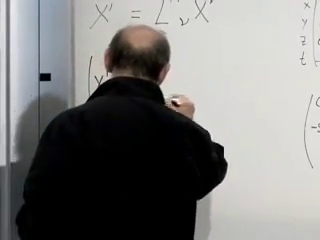
\includegraphics[width=0.8\textwidth]{lecture_06_figure_03.png}
\caption{Контравариантные и ковариантные компоненты, матрица метрики и начало инвариантной свёртки.}
\lectureframe{00:45:00}
\end{figure}

Понижение индекса — не украшение. Оно собирает знаки, необходимые для лоренц-инвариантной нормы:
\begin{align}
  A_\mu A^\mu
  &=-(A^1)^2-(A^2)^2-(A^3)^2+(A^0)^2,                    \label{eq:l6-norm}\\
  X_\mu X^\mu
  &=t^2-x^2-y^2-z^2.
\end{align}
Второе выражение есть инвариантный интервал пространства-времени от начала координат. Поскольку \(A^\mu\) преобразуется так же, как \(X^\mu\), его свёртка обладает той же инвариантностью.

Эта запись также подсказывает полезное правило учёта. Повторяющийся индекс суммирования встречается один раз вверху и один раз внизу. Например,
\begin{equation}
  A_\mu A^\mu
  =\eta_{\mu\nu}A^\mu A^\nu.
\end{equation}
Обозначения суммируемых, или фиктивных, индексов можно менять, не изменяя самой величины.

\begin{classroomqa}
\audiencequestion{Следует ли считать один из этих векторов строкой, а другой столбцом, и имеет ли значение их порядок?}
\lecturerresponse{В данном вычислении рассматривайте индексированные величины как компоненты и предоставьте метрике выполнить свёртку; нет нужды превращать обсуждение в операторную алгебру строк и столбцов. Это обычные числа, поэтому их порядок не имеет значения. Для некоммутирующих операторов потребовалась бы бо́льшая осторожность, но здесь речь не об этом.}
\end{classroomqa}

Та же конструкция задаёт скалярное произведение двух различных четырёхвекторов,
\begin{equation}
  A\mathbin{\cdot}B=A_\mu B^\mu=A^\mu B_\mu.
\end{equation}
Его инвариантность следует без явной записи матрицы Лоренца. Поскольку \(A+B\) и \(A-B\) являются четырёхвекторами, оба квадрата их норм инвариантны:
\begin{align}
  (A+B)^2&=A^2+B^2+2A\mathbin{\cdot}B,\\
  (A-B)^2&=A^2+B^2-2A\mathbin{\cdot}B.
\end{align}
Вычитая, получаем
\begin{equation}
  (A+B)^2-(A-B)^2=4A\mathbin{\cdot}B,                    \label{eq:l6-polarization}
\end{equation}
поэтому \(A\mathbin{\cdot}B\) тоже инвариантно. Множитель четыре следует непосредственно из разложения.\editorialnote{Вывод у доски даёт это поляризационное тождество; явная запись множителя делает озвученное сокращение недвусмысленным.}

\begin{figure}[H]
\centering
\includegraphics[width=0.8\textwidth]{lecture_06_figure_04.png}
\caption{Два инвариантных квадрата, используемые для выделения скалярного произведения различных четырёхвекторов.}
\lectureframe{00:52:20}
\end{figure}

Инвариантные величины естественно входят в физические законы: в отличие от отдельной компоненты, они сохраняют одно и то же значение при переходе от одной системы отсчёта к другой.

\section{Собственная скорость и четырёхимпульс}

Рассмотрим два соседних события на мировой линии частицы. Их разделяет бесконечно малый четырёхвектор
\begin{equation}
  dX^\mu=(dx,dy,dz,dt).
\end{equation}
Для времениподобной мировой линии собственное время определяется как
\begin{equation}
  d\tau^2=dX_\mu dX^\mu
  =dt^2-dx^2-dy^2-dz^2.                                  \label{eq:l6-proper-time}
\end{equation}
Собственная четырёхскорость равна
\begin{equation}
  U^\mu=\frac{dX^\mu}{d\tau}.                            \label{eq:l6-four-velocity}
\end{equation}
Она измеряет скорость изменения положения в пространстве-времени по собственному времени самой частицы, а не по координатному времени выбранной системы отсчёта.

Хотя \(U^\mu\) имеет четыре компоненты, независимы только три. Разделив ~\eqref{eq:l6-proper-time} на \(d\tau^2\), получаем
\begin{equation}
  U_\mu U^\mu=1.
\end{equation}
Следовательно, четырёхскорость является единичным времениподобным вектором. Выбор направления в будущее фиксирует знак её временной компоненты.

\begin{classroomqa}
\audiencequestion{При скоростях, много меньших \(c\), сводится ли четырёхскорость к обычной скорости?}
\lecturerresponse{Её три пространственные компоненты стремятся к обычной скорости, тогда как временная компонента стремится к единице в единицах \(c=1\). Это соотношение следует из применения правила дифференцирования сложной функции и вычисления \(dt/d\tau\).}
\end{classroomqa}

Для каждой пространственной компоненты
\begin{equation}
  U^i=\frac{dx^i}{d\tau}
     =\frac{dx^i}{dt}\frac{dt}{d\tau}
     =v^i\frac{dt}{d\tau}.
\end{equation}
Разделим ~\eqref{eq:l6-proper-time} на \(dt^2\):
\begin{equation}
  \left(\frac{d\tau}{dt}\right)^2
  =1-v_x^2-v_y^2-v_z^2
  =1-\boldsymbol v^2.
\end{equation}
Следовательно,
\begin{equation}
  \frac{dt}{d\tau}=\frac{1}{\sqrt{1-\boldsymbol v^2}}
  =\gamma(\lvert\boldsymbol v\rvert),
\end{equation}
и
\begin{equation}
  U^\mu=(\gamma v_x,\gamma v_y,\gamma v_z,\gamma).
                                                                  \label{eq:l6-u-components}
\end{equation}

\begin{figure}[H]
\centering
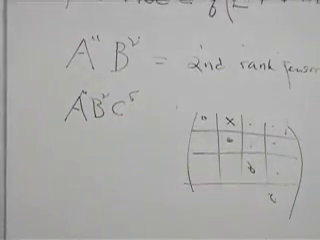
\includegraphics[width=0.8\textwidth]{lecture_06_figure_05.png}
\caption{Вычисление собственного времени, которое даёт \(dt/d\tau=\gamma\) и связывает собственную скорость с обычной скоростью.}
\lectureframe{01:02:00}
\end{figure}

\begin{classroomqa}
\audiencequestion{Означает ли \(dx^2/dt^2\) вторую производную, и должны ли при возведении вектора в квадрат возникать перекрёстные члены?}
\lecturerresponse{Здесь это означает \((dx/dt)^2\), квадрат первой производной. Кроме того, \(\boldsymbol v^2\) означает евклидово скалярное произведение \(v_x^2+v_y^2+v_z^2\), а не квадрат формальной суммы \(v_x+v_y+v_z\); перекрёстных членов нет.}
\end{classroomqa}

\begin{classroomqa}
\audiencequestion{Является ли \(v\) в \(\gamma(v)\) относительной скоростью двух систем отсчёта или скоростью частицы?}
\lecturerresponse{Здесь это скорость частицы в выбранной системе отсчёта. Функцию \(\gamma(v)=1/\sqrt{1-v^2}\) можно вычислять для любой скорости: при бусте она вычисляется на относительной скорости систем отсчёта; в четырёхскорости — на скорости частицы.}
\end{classroomqa}

Для \(v\ll1\), \(\gamma\simeq1\), поэтому пространственные компоненты \(U^\mu\) стремятся к \(\boldsymbol v\), а \(U^0\) стремится к единице. Когда обычная скорость приближается к скорости света, \(\gamma\) и все ненулевые компоненты четырёхскорости растут без ограничения.

\begin{classroomqa}
\audiencequestion{Не должна ли \(U^0\) иметь размерность скорости, вместо того чтобы быть близкой к числу один?}
\lecturerresponse{Размерности исчезли, когда \(c\) было положено равным единице. При \(X^0=ct\) имеем
\(U^\mu=(\gamma\boldsymbol v,\gamma c)\), так что временная компонента стремится к \(c\), и \(U_\mu U^\mu=c^2\).}
\end{classroomqa}

Для частицы с массой покоя \(m\) определим четырёхимпульс как
\begin{equation}
  P^\mu=mU^\mu.
\end{equation}
В естественных единицах
\begin{equation}
  P^\mu=(\gamma m\boldsymbol v,\gamma m).
\end{equation}
Первые три компоненты при малой скорости стремятся к ньютоновскому импульсу \(m\boldsymbol v\). Восстанавливая единицы, получаем
\begin{equation}
  P^\mu=(\gamma m\boldsymbol v,E/c),
  \qquad E=\gamma mc^2,
\end{equation}
и, следовательно,
\begin{equation}
  E=mc^2+\frac{1}{2}m\boldsymbol v^2+O(mv^4/c^2).
\end{equation}
Временная компонента есть энергия в единицах \(c=1\) или энергия, делённая на \(c\), когда всем четырём компонентам приписываются единицы импульса.

\begin{classroomqa}
\audiencequestion{Является ли обычная \(\boldsymbol v\), если дописать к ней четвёртую компоненту, сама по себе четырёхвектором?}
\lecturerresponse{Нет. Обычная трёхскорость не преобразуется как четырёхвектор. Множитель \(\gamma\) и определение через собственное время существенны; четырёхвектор — это \(U^\mu\), а не \(\boldsymbol v\).}
\end{classroomqa}

\section{Почему электрическое и магнитное поля должны смешиваться}

Теперь вернёмся к тому, что было названо кратким отпуском от относительности. Начнём с доэйнштейновского уравнения движения и спросим, как его нужно перестроить, чтобы оно могло быть справедливым в любой инерциальной системе отсчёта. Обычное ускорение есть производная обычной скорости по времени. Его четырёхмерным аналогом естественно является
\begin{equation}
  A^\mu=\frac{dU^\mu}{d\tau}.
\end{equation}
При малой скорости его пространственные компоненты стремятся к обычному ускорению. Полное релятивистское уравнение будет отложено; сначала рассмотрим старый закон силы.

Для заряда \(q\) в электрическом и магнитном полях
\begin{equation}
  \boldsymbol F=m\boldsymbol a
  =q\left(\boldsymbol E+\boldsymbol v\times\boldsymbol B\right).
                                                                  \label{eq:l6-lorentz-force}
\end{equation}
Электрический член не зависит от скорости частицы, тогда как магнитный зависит.

\begin{figure}[H]
\centering
\includegraphics[width=0.8\textwidth]{lecture_06_figure_06.png}
\caption{Дорелятивистская форма закона силы Лоренца, которая мотивирует объединение \(\boldsymbol E\) и \(\boldsymbol B\).}
\lectureframe{01:18:20}
\end{figure}

Предположим, наблюдатель не видит электрического поля, но видит магнитное поле и движущийся заряд. Заряд испытывает магнитную силу. Однако в мгновенной системе покоя заряда \(\boldsymbol v=0\), поэтому магнитный член в ~\eqref{eq:l6-lorentz-force} обращается в нуль. Физическая мировая линия не стала инерциальной лишь потому, что изменились координаты; следовательно, сила в новой системе должна включать электрический вклад. Точнее, ненулевое четырёхускорение нельзя преобразованием между инерциальными системами обратить в нуль, хотя трёхускорение и его компоненты преобразуются.
\editorialnote{Это утверждение о четырёхускорении является инвариантной формой аудиторного аргумента и позволяет не трактовать обычное трёхускорение само по себе как инвариант относительно системы отсчёта.}

Следовательно, электрическое и магнитное поля должны преобразовываться друг в друга. Вместе у них шесть компонент, поэтому они не являются ни одним скаляром, ни одним четырёхвектором. Нам нужен новый объект с собственным законом преобразования.

\section{Тензоры: по одному преобразованию на индекс}

Скаляр можно назвать тензором ранга нуль; у него нет индексов. Четырёхвектор — тензор ранга один; у него один индекс с четырьмя возможными значениями. Простейший пример ранга два — произведение
\begin{equation}
  A^\mu B^\nu.
\end{equation}
Каждый индекс принимает четыре значения, поэтому у объекта \(4^2=16\) компонент, которые можно представить в виде массива \(4\times4\). Произведение трёх векторов,
\begin{equation}
  A^\mu B^\nu C^\sigma,
\end{equation}
имеет \(4^3=64\) компонент и является тензором ранга три. Для более высоких рангов схема продолжается. Название менее важно, чем правило, которым определяется объект.

Если
\begin{equation}
  A'^{\mu}=\Lambda^\mu{}_{\nu}A^\nu,
  \qquad
  B'^{\sigma}=\Lambda^\sigma{}_{\tau}B^\tau,
\end{equation}
то их произведение преобразуется как
\begin{equation}
  A'^{\mu}B'^{\sigma}
  =\Lambda^\mu{}_{\nu}\Lambda^\sigma{}_{\tau}
   A^\nu B^\tau.
\end{equation}
Это даёт определяющий закон для контравариантного тензора ранга два:
\begin{equation}
  T'^{\mu\sigma}
  =\Lambda^\mu{}_{\nu}\Lambda^\sigma{}_{\tau}T^{\nu\tau}.
                                                                  \label{eq:l6-tensor-transform}
\end{equation}
Каждому индексу соответствует одна матрица Лоренца. Повторяющиеся \(\nu\) и \(\tau\) суммируются; свободные \(\mu\) и \(\sigma\) обозначают компоненту, вычисляемую в штрихованной системе отсчёта.

\begin{figure}[H]
\centering
\includegraphics[width=0.82\textwidth]{lecture_06_figure_07.png}
\caption{Преобразование двух векторов и вытекающий из него двухматричный закон преобразования тензора ранга два.}
\lectureframe{01:27:15}
\end{figure}

Тензор не обязан быть одиночным произведением векторов. И \(A^\mu B^\nu\), и \(A^\nu B^\mu\) подчиняются тензорному закону преобразования, как и их сумма и любая сумма вида
\begin{equation}
  A^\mu B^\nu+C^\mu D^\nu.
\end{equation}
Определением служит закон преобразования, а не конкретная факторизация. Тензор третьего ранга получает третью матрицу Лоренца, и так далее.

\section{Симметричные и антисимметричные тензоры}

Два класса тензоров ранга два будут особенно полезны. Симметричный тензор удовлетворяет
\begin{equation}
  T^{\mu\nu}=T^{\nu\mu},
\end{equation}
так что элементы, отражённые относительно диагонали, совпадают. Его четыре диагональных элемента и шесть элементов по одну сторону диагонали определяют остальные, давая
\begin{equation}
  4+6=10
\end{equation}
независимых компонент.

Антисимметричный тензор удовлетворяет
\begin{equation}
  T^{\mu\nu}=-T^{\nu\mu}.                                \label{eq:l6-antisymmetry}
\end{equation}
Подстановка \(\mu=\nu\) в ~\eqref{eq:l6-antisymmetry} даёт
\(T^{\mu\mu}=-T^{\mu\mu}\), так что каждый диагональный элемент равен нулю. Шесть элементов в одной треугольной половине определяют остальные шесть изменением знака. Поэтому имеется ровно шесть независимых компонент.

\begin{figure}[H]
\centering
\includegraphics[width=0.82\textwidth]{lecture_06_figure_08.png}
\caption{Заполненный антисимметричный массив \(4\times4\): нули на диагонали и противоположные знаки по разные стороны от неё.}
\lectureframe{01:34:25}
\end{figure}

Именно это число и служит подсказкой. Три электрические и три магнитные компоненты могут поместиться в один антисимметричный тензор ранга два.

\section{Тензор электромагнитного поля}

Пусть метки пространства-времени идут по строкам и столбцам в порядке
\((1,2,3,0)=(x,y,z,t)\). Запись на доске имеет вид
\begin{equation}
  F_{\mu\nu}=
  \begin{pmatrix}
    0    & -B_3 & B_2  & E_1\\
    B_3  & 0    & -B_1 & E_2\\
    -B_2 & B_1  & 0    & E_3\\
    -E_1 & -E_2 & -E_3 & 0
  \end{pmatrix}.                                         \label{eq:l6-field-tensor}
\end{equation}
Чисто пространственные ячейки содержат магнитное поле; ячейки с одним пространственным и одним временным индексом содержат электрическое поле. Антисимметрия задаёт элементы нижнего треугольника, как только известны элементы верхнего треугольника.

\begin{classroomqa}
\audiencequestion{Все ли магнитные элементы отрицательны, и соответствуют ли метки \(x,y,z\)?}
\lecturerresponse{Знаки в верхнем пространственном треугольнике чередуются так, как показано: \(-B_3,+B_2,-B_1\). Метки \(1,2,3\) соответствуют \(x,y,z\), тогда как \(0\) обозначает время. При отражении относительно диагонали каждый знак меняется на противоположный.}
\end{classroomqa}

\begin{figure}[H]
\centering
\includegraphics[width=0.82\textwidth]{lecture_06_figure_09.png}
\caption{Полный тензор электромагнитного поля в используемом в лекции порядке компонент, где пространственные компоненты идут первыми.}
\lectureframe{01:41:05}
\end{figure}

Обозначение по соглашению пишут как \(F_{\mu\nu}\), а не как общее
\(T_{\mu\nu}\). Лектор предполагает, что буква может отсылать к
Фарадею, одновременно прямо говоря, что не знает истории этого
обозначения. Здесь важны его антисимметрия и шесть компонентов поля,
а не это предположение о букве.

\begin{classroomqa}
\audiencequestion{Представляет ли каждый элемент матрицы величину поля в указанной координатной плоскости?}
\lecturerresponse{Это компонента тензора электромагнитного поля.
Элементы, содержащие время, являются электрическими компонентами, а пространственные--пространственные
элементы кодируют магнитные компоненты.}
\end{classroomqa}

Отделите строку и столбец, несущие временной индекс. Оставшийся
антисимметричный блок \(3\times3\) соответствует магнитному полю. Его независимые элементы удобно
запоминать циклически:
\begin{equation}
  F_{12}=-B_3,
  \qquad F_{23}=-B_1,
  \qquad F_{31}=-B_2.                                   \label{eq:l6-magnetic-cycle}
\end{equation}
Начиная с первого соотношения, циклически сдвигайте все метки по
\(1\to2\to3\to1\). Эквивалентно,
\begin{equation}
  F_{ij}=-\epsilon_{ijk}B_k,
\end{equation}
где \(\epsilon_{123}=+1\).\editorialnote{Формула Леви--Чивиты — компактная стандартная форма циклического правила, явно выведенного на доске.}

\begin{figure}[H]
\centering
\includegraphics[width=0.82\textwidth]{lecture_06_figure_10.png}
\caption{Циклические пространственные компоненты, кодирующие магнитное поле в антисимметричном тензоре.}
\lectureframe{01:46:20}
\end{figure}

Для электрического поля соответствия более прямые:
\begin{equation}
  E_1=F_{10},
  \qquad E_2=F_{20},
  \qquad E_3=F_{30}.
\end{equation}

Поэтому для магнитного поля полезны два отождествления. Внутри
трёхмерного пространства трёхкомпонентному аксиальному вектору можно
поставить в соответствие антисимметричный тензор \(3\times3\). В пространстве-времени,
однако, оно является лишь пространственной частью шестикомпонентного тензора
\(F_{\mu\nu}\). Такое сопоставление специфично для трёх измерений:
антисимметричный тензор \(4\times4\) имеет шесть независимых компонент и не
может быть отождествлён с четырёхвектором.
\editorialnote{При собственных вращениях магнитное поле ведёт себя как вектор;
при отражениях, точнее, как аксиальный вектор, или псевдовектор.}

Цель этой конструкции не в подсчёте компонент как таковом.
Поскольку \(F_{\mu\nu}\) преобразуется как тензор, буст Лоренца автоматически
смешивает его электрические и магнитные элементы. На следующей лекции его
можно будет объединить с четырёхскоростью и четырёхускорением, чтобы заменить
уравнение~\eqref{eq:l6-lorentz-force} ковариантным уравнением движения.

\section{Вопросы об Эйнштейне и Минковском}

В последние минуты разговор переходит от формализма к тому, как он возник исторически. Ответы даются как воспоминания, а не как установленная история, и эта оговорка сама является частью обсуждения.

\begin{classroomqa}
\audiencequestion{Искал ли Эйнштейн лоренц-инвариантную формулировку из концептуальных соображений, или его к ней вели конкретные наблюдения?}
\lecturerresponse{Принцип, согласно которому законы природы должны иметь одну и ту же форму во всякой инерциальной системе отсчёта, был центральным в его рассуждениях. Были также экспериментальные данные, касающиеся света и невозможности обнаружить движение сквозь эфир, хотя лектор прямо не уверен, какие именно результаты были известны Эйнштейну и насколько сильно они на него повлияли. Концептуальное требование состояло в том, что уравнения Максвелла и сила Лоренца должны подчиняться принципу относительности, а это требует, чтобы электрические поля, магнитные поля и компоненты скорости преобразовывались совместно.}
\end{classroomqa}

В изложении Эйнштейна 1905 года не использовалась компактная нотация четырёхвекторов,
используемая здесь. Там всё делалось покомпонентно, с явной записью необходимых
множителей \(\gamma\) и скорости. Минковский впоследствии организовал ту же
структуру геометрически как четырёхмерное пространство-время.

\begin{classroomqa}
\audiencequestion{Сопротивлялся ли Эйнштейн простран\-ственно-временной формулировке Минковского, и как скоро Минковский её ввёл?}
\lecturerresponse{Высказанное на занятии воспоминание состоит в том, что Эйнштейн поначалу не приветствовал четырёхмерный геометрический язык, но быстро оценил его ценность. Время указывается предположительно как примерно через два года после статьи 1905 года, возможно 1907; выступающий подчёркивает, что он вспоминает, а не устанавливает историю.}
\end{classroomqa}

\begin{classroomqa}
\audiencequestion{Был ли Минковский математиком или физиком, что ещё он внёс, и испытывал ли он влияние Лоренца или Фицджеральда?}
\lecturerresponse{Никакого уверенного ответа не даётся. Различие между математиком и физиком не разбиралось, поправка из аудитории прерывает общее замечание о других работах Минковского, а возможные линии влияния прямо оставляются неопределёнными. Надёжный пункт для этого обсуждения состоит в том, что Минковский решающим образом оформил теорию относительности в четырёхмерной геометрической нотации.}
\end{classroomqa}

\begin{classroomqa}
\audiencequestion{Присутствовали ли преобразования, смешивающие \(\boldsymbol E\) и
\(\boldsymbol B\), уже в работе Эйнштейна 1905 года?}
\lecturerresponse{Да, но они были записаны покомпонентно, а не как одно
уравнение полевого тензора. Проведённое на занятии сравнение — с покомпонентными
уравнениями Максвелла: содержание может присутствовать и до появления компактной
нотации, раскрывающей его общую структуру. Вклад Минковского состоял в том,
чтобы сделать эту структуру систематической на языке пространства-времени.}
\end{classroomqa}

Это возвращает нас к математической мысли, с которой мы начали. Компоненты незаменимы для вычислений, но закон становится понятным, когда эти компоненты распознаются как части единого преобразующегося объекта. Следующая задача — использовать \(F_{\mu\nu}\), чтобы записать уравнение движения заряженной частицы в форме, одинаковой во всех инерциальных системах отсчёта.
